%\documentclass[a4paper,twoside,11pt,open=any]{scrbook}
%damit die erste Seite einer Übung immer links gelocht ist:
\documentclass[a4paper,11pt,open=any]{scrbook}

\usepackage{fancyhdr}

\usepackage[utf8]{inputenc}			%für deutsche Sonderzeichen
%\usepackage[ngerman]{babel}			%für deutsches Datum
\usepackage[UKenglish]{babel}
%\usepackage[babel,german=quotes]{csquotes}	%deutsche Anführungszeichen
\usepackage[T1]{fontenc}			%für Umlaute und Akzente
\usepackage{graphicx}				%für Grafiken
\usepackage{newcent}				%für Skalierbarkeit der Schrift
\usepackage{amsmath}				%Verbesserung der Formeln
\usepackage{amssymb}
\usepackage{cancel}					%kürzen in Formeln
\usepackage{ulem}					%für Unterstrich
\usepackage{enumitem} 				%Aufzählungen


\usepackage{geometry}
\geometry{a4paper,left=25mm,right=15mm, top=10mm, bottom=25mm}

\geometry{left=25mm, right=10mm}
\geometry{top=30mm,bottom=30mm}
\geometry{headheight=20mm}
\geometry{headsep=5mm}
\geometry{footskip=10mm} 


\usepackage {tikz}
\usetikzlibrary {positioning}
\usepackage{url}
\usepackage{xcolor}
\definecolor{white} {rgb}{255, 255, 255}
\definecolor{red} {rgb}{255, 0, 0}
\usepackage[pdfstartview=FitBH, breaklinks = true, citebordercolor = white, linkbordercolor = white, urlbordercolor  = white]{hyperref}
\hypersetup
{
	pdftitle = {Robotics Lehmann & Bullmann}
	pdfsubject = {Robotics Lehmann & Bullmann},
	pdfkeywords = {LaTeX, robotics, Tutorium, \"Ubungszettel},
	pdfauthor = {Tom Bullmann},
}

%\renewcommand \thechapter {\arabic{chapter}.\hspace{0.5em}}
%\renewcommand \thesection {\arabic{chapter}.\arabic{section}:}
%\renewcommand \thesubsection {\arabic{chapter}.\arabic{section}.\arabic{subsection}:}
\usepackage{tocloft} 
\setlength{\cftsecnumwidth}{5.5em} % damit der lange String "Aufgabe 1" passt

\addto\captionsUKenglish{%
\renewcommand{\contentsname}{Table of Contents}}
\renewcommand*\chapterheadstartvskip{\vspace*{0mm}}


\usepackage{listings}
\lstset{language=C,numbers=left,xleftmargin=10mm
,commentstyle=\small\selectfont,basicstyle=\ttfamily\small\selectfont,
    frame=single,
    breaklines=true,
    postbreak=\raisebox{0ex}[0ex][0ex]{\ensuremath{\color{red}\hookrightarrow\space}}
}

\usepackage{tabularx}

%\lstset{}

	\fancypagestyle{plain}{
		\fancyhf{}
		\fancyhead[OL,ER]{WS 15/16 \\ \today}
		\fancyhead[C]{\textbf{Robotics}  \\ Lecturer: Prof. Dr. Daniel G\"ohring }
    \fancyhead[OR,EL]{Tom Bullmann \begin{tiny}(4280486)\end{tiny}\\
    Nicolas Lehmann \begin{tiny}(4093195)\end{tiny} }
		\renewcommand{\headrulewidth}{0.4pt} %obere Trennlinie
		\fancyfoot[OR,EL]{\smallskip \thepage} %Seitennummer
		\fancyfoot[C]{\tiny{Free Univertiy of Berlin\\Department of Mathematics and Computer Science\\Institute of Computer Science}}
		\renewcommand{\footrulewidth}{0.4pt} %untere Trennlinie
	}

\begin{document}
  \pagestyle{plain}
  \begin{titlepage}
  \begin{center}
    \Large
    \textsc
    {
    	\\
    	\vspace{2cm}
    	Robotics
    }\\
  	\vspace{5cm}
  	\textsc
  	{
  		Assignment 13\\[0.5\baselineskip]
  		by\\[0.5\baselineskip]
  		Tom Bullmann and Nicolas Lehmann
  	}\\
  	\vspace{5cm}
    \textsc{\today}\\
    \vspace{1cm}
    \textsc
    {
    	Lecturer:\\
    	Prof. Dr. Daniel G\"ohring
    }\\
  	\vspace{1cm}
  	\textsc{
  		Free Univertiy of Berlin\\
  		Department of Mathematics and Computer Science\\
  		Institute of Computer Science
  	}\\
  \end{center}
\end{titlepage}
  \pagenumbering{Roman}
  \tableofcontents
  \clearpage
  \pagenumbering{arabic}
  %\chapter{Assignment 1}\label{ass1}

\section{Task 1}\label{ass1_t1}

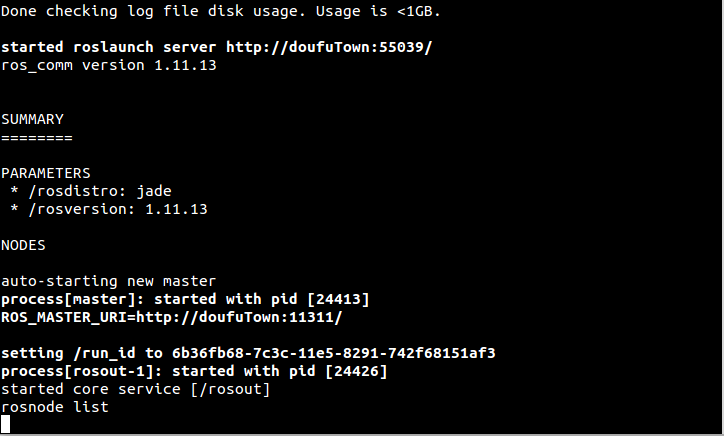
\includegraphics{img/screen_ue1_t1.png}

\section{Task 2}\label{ass1_t2}

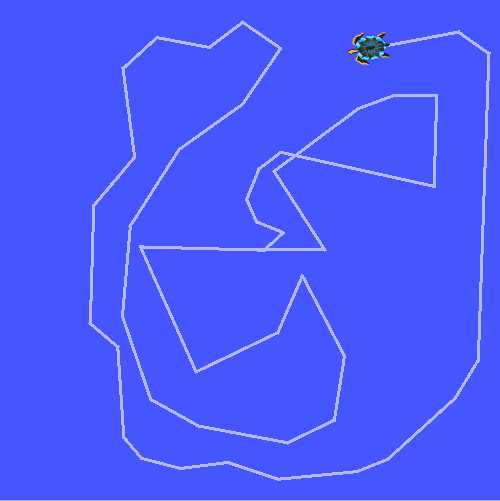
\includegraphics{img/screen_ue1_t2.png}
  %\chapter{Assignment 2}\label{ass2}

\section{Task 1}\label{ass2_t1}

\subsection{a}\label{ass2_t1_a}

\begin{equation}
  \begin{pmatrix}
    x_{1} \\
    y_{1}
  \end{pmatrix}
  =
  \begin{pmatrix}
    cos(\Theta_{1})  &  sin(\Theta_{1}) \\
    -sin(\Theta_{1}  &  cos(\Theta_{1}
  \end{pmatrix}
  \cdot
  \begin{pmatrix}
    L_{1} \\
    0
  \end{pmatrix}
  =
  \begin{pmatrix}
    L_{1}\cdot cos(\Theta_{1})   & 0 \\
    -L_{1}\cdot sin(\Theta_{1})  & 0
  \end{pmatrix}
  =
  \begin{pmatrix}
    L_{1}\cdot cos(\Theta_{1}) \\
    -L_{1}\cdot sin(\Theta_{1})
  \end{pmatrix}
\end{equation}

With $(x_{1}, y_{1})$ calculated in correlation to $(x, y)$, we assume $(x_{1}, y_{1})$ as the new start to calculate $(x_{2}, y_{2})$.

\begin{equation}
  \begin{pmatrix}
    x_{2} \\
    y_{2}
  \end{pmatrix}
  =
  \begin{pmatrix}
    cos(\Theta_{2})  &  -sin(\Theta_{2}) \\
    sin(\Theta_{2}  &  cos(\Theta_{2}
  \end{pmatrix}
  \cdot
  \begin{pmatrix}
    L_{2} \\
    0
  \end{pmatrix}
  =
  \begin{pmatrix}
    L_{2}\cdot cos(\Theta_{2})   & 0 \\
    L_{2}\cdot sin(\Theta_{2})  & 0
  \end{pmatrix}
  =
  \begin{pmatrix}
    L_{2}\cdot cos(\Theta_{2}) \\
    L_{2}\cdot sin(\Theta_{2})
  \end{pmatrix}
\end{equation}

\subsection{b}\label{ass2_t1_b}

The four euqations are: $x_{1} = L_{1}\cdot cos(\Theta_{1})$, $y_{1} = L_{1}\cdot sin(\Theta_{1})$, $x_{2} = L_{2}\cdot cos(\Theta_{2})$ and $y_{2} = L_{2}\cdot sin(\Theta_{2})$.
\begin{equation}
  \frac{x_{1}}{d\Theta_{1}} = -L_{1}\cdot sin(\Theta_{1})
\end{equation}
\begin{equation}
  \frac{x_{1}}{d\Theta_{2}} = 0
\end{equation}
\begin{equation}
  \frac{y_{1}}{d\Theta_{1}} = -L_{1}\cdot cos(\Theta_{1})
\end{equation}
\begin{equation}
  \frac{y_{1}}{d\Theta_{2}} = 0
\end{equation}
\begin{equation}
  \frac{x_{2}}{d\Theta_{1}} = 0
\end{equation}
\begin{equation}
  \frac{x_{2}}{d\Theta_{2}} = -L_{2}\cdot sin(\Theta_{2})
\end{equation}
\begin{equation}
  \frac{y_{2}}{d\Theta_{1}} = 0
\end{equation}
\begin{equation}
  \frac{y_{2}}{d\Theta_{2}} = L_{2}\cdot cos(\Theta_{2})
\end{equation}


\section{Task 2}\label{ass2_t2}

\subsection{a}\label{ass2_t2_a}



\subsection{b+c}\label{ass2_t2_b_c}

The coordinates have been marked in the following picture by a red eclipse.

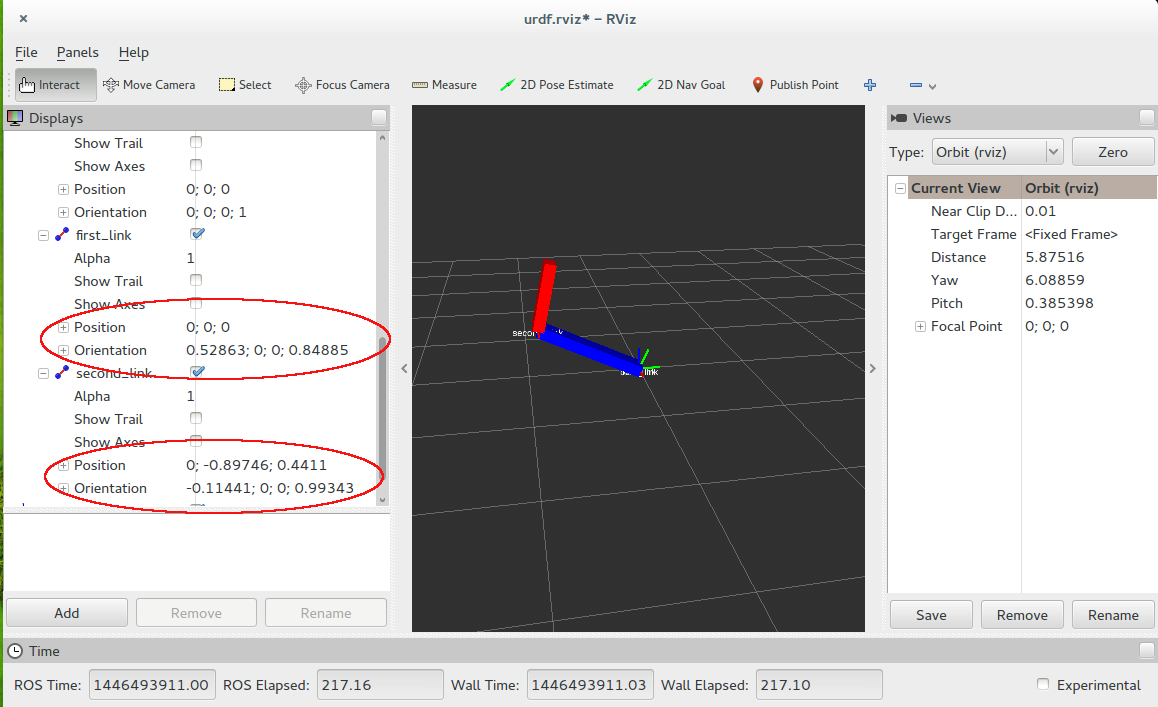
\includegraphics[width=\textwidth]{img/screen_ue2_t2_c.png}


  %\chapter{Assignment 3}\label{ass3}

\section{Task 1}\label{ass3_t1}

\subsection{a}\label{ass3_t1_a}

We assume that the given vectors in \{A\} are unit vetors.

\begin{equation}
  ^{B}_{A}T
  =
  \begin{pmatrix}
    0   & -1  & 0   & -3  \\
    -1  & 0   & 0   & -2  \\
    0   & 0   & -1  & -2  \\
    0   & 0   & 0   & 1
  \end{pmatrix}
\end{equation}

\subsection{b}\label{ass3_t1_b}

\begin{equation}
  v_{B}
  =
  \begin{pmatrix}
    1 \\
    -2\\
    3
  \end{pmatrix}
\end{equation}
\begin{equation}
  ^{A}v_{B}
  =
  ^{B}_{A}T\cdot v_{B}
  =
  \begin{pmatrix}
    0   & -1  & 0   & -3  \\
    -1  & 0   & 0   & -2  \\
    0   & 0   & -1  & -2  \\
    0   & 0   & 0   & 1
  \end{pmatrix}
  \cdot
  \begin{pmatrix}
    1 \\
    -2\\
    3 \\
    1
  \end{pmatrix}
  =
  \begin{pmatrix}
    0\cdot 1  &+& -1\cdot -2 &+& 0\cdot 3  &+& -3\cdot 1 \\
    -1\cdot 1 &+& 0\cdot -2  &+& 0\cdot 3  &+& -2\cdot 1 \\
    0\cdot 1  &+& 0\cdot -2  &+& -1\cdot 3 &+& -2\cdot 1 \\
    0\cdot 1  &+& 0\cdot -2  &+& 0\cdot 3  &+& 1\cdot 1
  \end{pmatrix}
  =
  \begin{pmatrix}
    -1 \\
    -3\\
    -5 \\
    1
  \end{pmatrix}
\end{equation}


\section{Task 2}\label{ass3_t2}

\subsection{a}\label{ass3_t2_a}

Output from the talker/chatter:
\begin{lstlisting}
[ INFO] [1447112923.955038907]: count: 1, Random number: 83
[ INFO] [1447112923.955403754]: count: 2, oldNumber: 83, incoming number: 182, outgoing number: 265
[ INFO] [1447112924.955113306]: count: 3, oldNumber: 265, incoming number: 530, outgoing number: 795
[ INFO] [1447112924.956239674]: count: 4, oldNumber: 795, incoming number: 1325, outgoing number: 2120
[ INFO] [1447112924.957031112]: count: 5, oldNumber: 2120, incoming number: 3445, outgoing number: 5565
[ INFO] [1447112924.957963184]: count: 6, oldNumber: 5565, incoming number: 9010, outgoing number: 14575
[ INFO] [1447112924.958748419]: count: 7, oldNumber: 14575, incoming number: 23585, outgoing number: 38160
[ INFO] [1447112924.959570396]: count: 8, oldNumber: 38160, incoming number: 61745, outgoing number: 99905
[ INFO] [1447112924.960333586]: count: 9, oldNumber: 99905, incoming number: 161650, outgoing number: 261555
[ INFO] [1447112924.961155844]: count: 10, oldNumber: 261555, incoming number: 423205, outgoing number: 684760
\end{lstlisting}

Output from the listener:
\begin{lstlisting}
[ INFO] [1447112922.956032343]: count: 1, oldNumber: 99, incoming number: 83, outgoing number: 182
[ INFO] [1447112923.955724576]: count: 2, oldNumber: 182, incoming number: 83, outgoing number: 265
[ INFO] [1447112923.955932006]: count: 3, oldNumber: 265, incoming number: 265, outgoing number: 530
[ INFO] [1447112924.955830461]: count: 4, oldNumber: 530, incoming number: 795, outgoing number: 1325
[ INFO] [1447112924.956670109]: count: 5, oldNumber: 1325, incoming number: 2120, outgoing number: 3445
[ INFO] [1447112924.957561409]: count: 6, oldNumber: 3445, incoming number: 5565, outgoing number: 9010
[ INFO] [1447112924.958415454]: count: 7, oldNumber: 9010, incoming number: 14575, outgoing number: 23585
[ INFO] [1447112924.959119514]: count: 8, oldNumber: 23585, incoming number: 38160, outgoing number: 61745
[ INFO] [1447112924.959956892]: count: 9, oldNumber: 61745, incoming number: 99905, outgoing number: 161650
[ INFO] [1447112924.960733532]: count: 10, oldNumber: 161650, incoming number: 261555, outgoing number: 423205
\end{lstlisting}

Source code is in the files listener.cpp and talker.cpp.

\subsection{b}\label{ass3_t2_b}

Unfortunately the display.launch from the arm2f repositiory could not be used to run the simulation, due to some error in the display.launch file it seems, therefore we were not able to solve this task.
  %\chapter{Assignment 4}\label{ass4}

\section{Task 1}\label{ass4_t1}

For input 1:\\
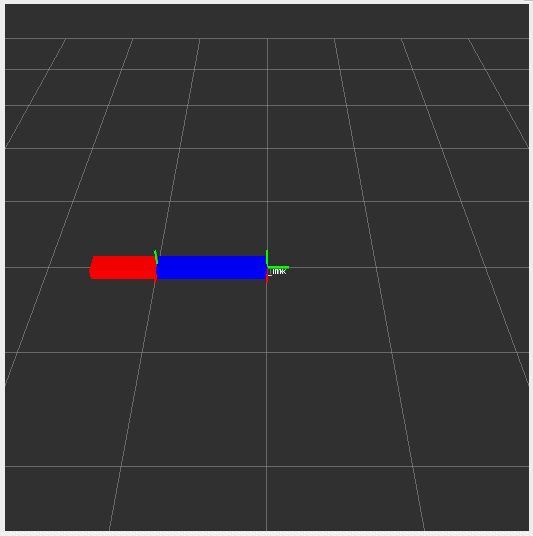
\includegraphics[width=0.75\textwidth]{img/screen_ue4_t1_1.png}
\newpage
For input 2:\\
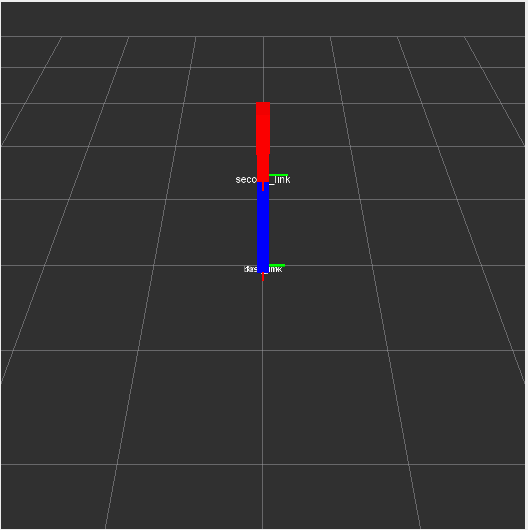
\includegraphics[width=0.75\textwidth]{img/screen_ue4_t1_2.png}
\newpage
For input 3:\\
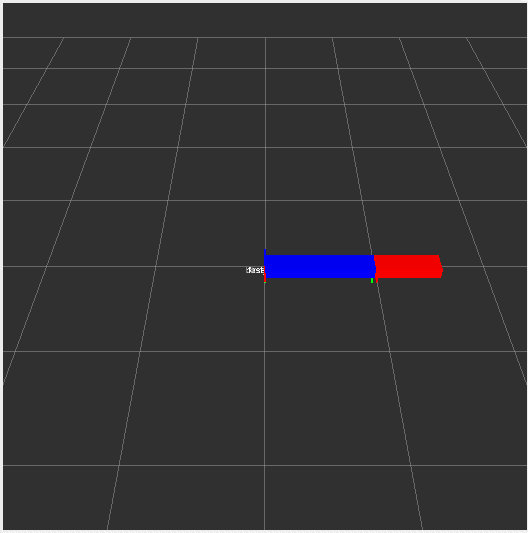
\includegraphics[width=0.75\textwidth]{img/screen_ue4_t1_3.png}

\section{Task 2}\label{ass4_t2}

\subsection{a}\label{ass4_t2a}

The robot as shown after concluding the first point in the README.md:\\
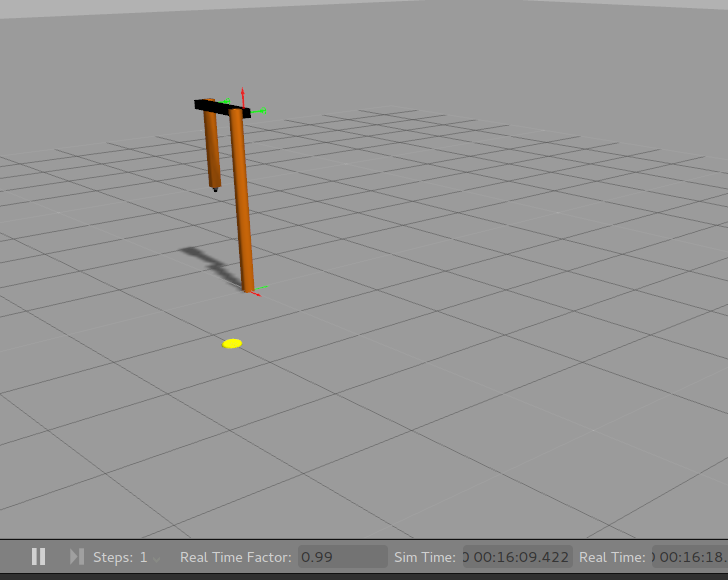
\includegraphics[width=0.75\textwidth]{img/screen_ue4_t2_a1.png}\\


We are not able to select 'Joint trajectory controller' as it is no option in the Robot Tools.
Our best guess is, it has to with the rrbot\_hw-package not compiling due to errors, as shown below.\\
Unfortunately we have no clue on how to rectify this error so, we can not change the robots joints.\\
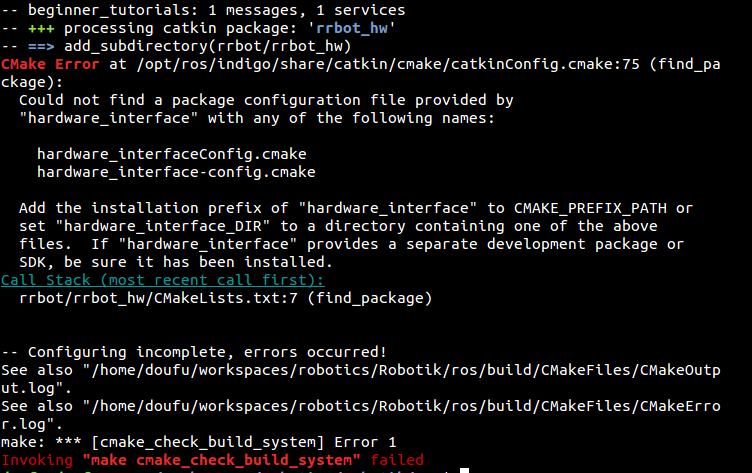
\includegraphics[width=0.75\textwidth]{img/screen_ue4_t2_a_1-fail.png}\\
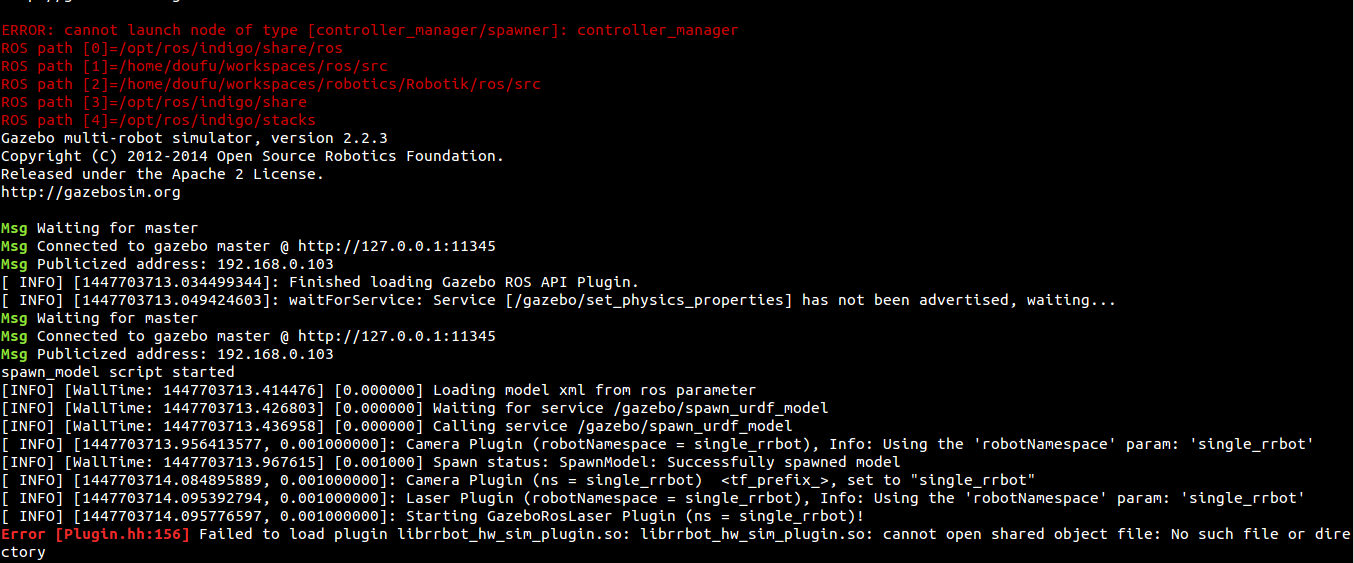
\includegraphics[width=0.75\textwidth]{img/screen_ue4_t2_a_2-fail.png}


\subsection{b}\label{ass4_t2b}

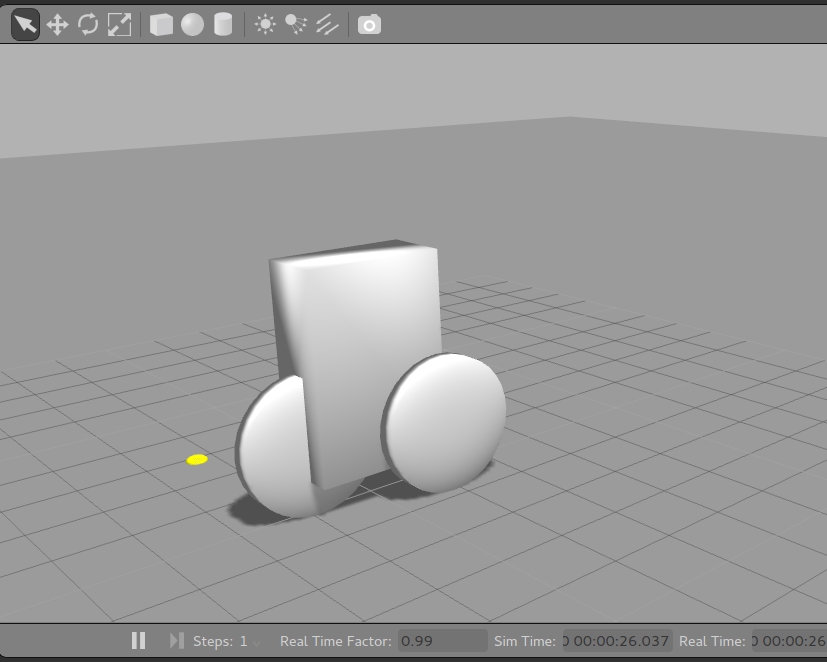
\includegraphics[width=0.75\textwidth]{img/screen_ue4_t2_b.png}

\subsection{Task 3}\label{ass4_t3}

Fixed-Angles: $- 90^\circ$ in Y-axis and then $90^\circ$ in X-axis.

\noindent ZYX-Euler-Angles: $(-90^\circ, 0^\circ, 90^\circ)$.

\noindent ZYZ-Euler-Angles: $(0^\circ, -90^\circ, -90^\circ)$.
  %\chapter{Assignment 5}\label{ass5}

\section{Task 1}\label{ass5_t1}

We already switched from jade to indigo for the last assignment, as can be seen in the attached picture from last week.

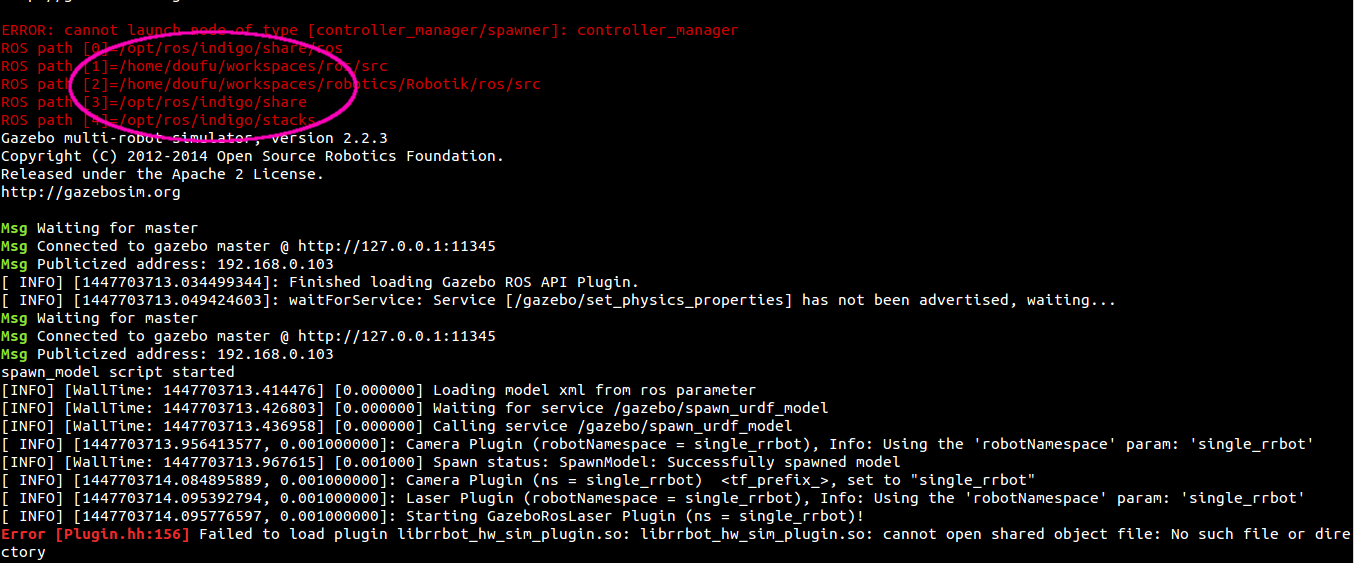
\includegraphics[width=0.75\textwidth]{img/screen_ue5_t1.png}

\section{Task 2}\label{ass5_t2}

Screenshot of the whole car:\\
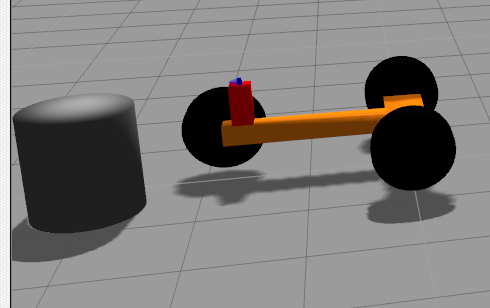
\includegraphics[width=0.75\textwidth]{img/screen_ue5_t2_car.png}\newpage

Screenshot of the camera-picture:\\
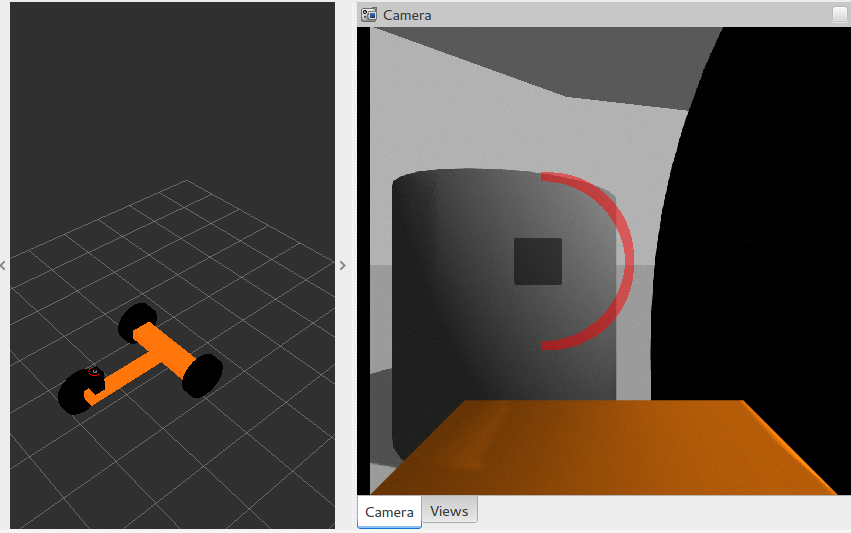
\includegraphics[width=0.75\textwidth]{img/screen_ue5_t2_cam.png}

Screenshot of the point cloud generated by the laser-scanner:\\
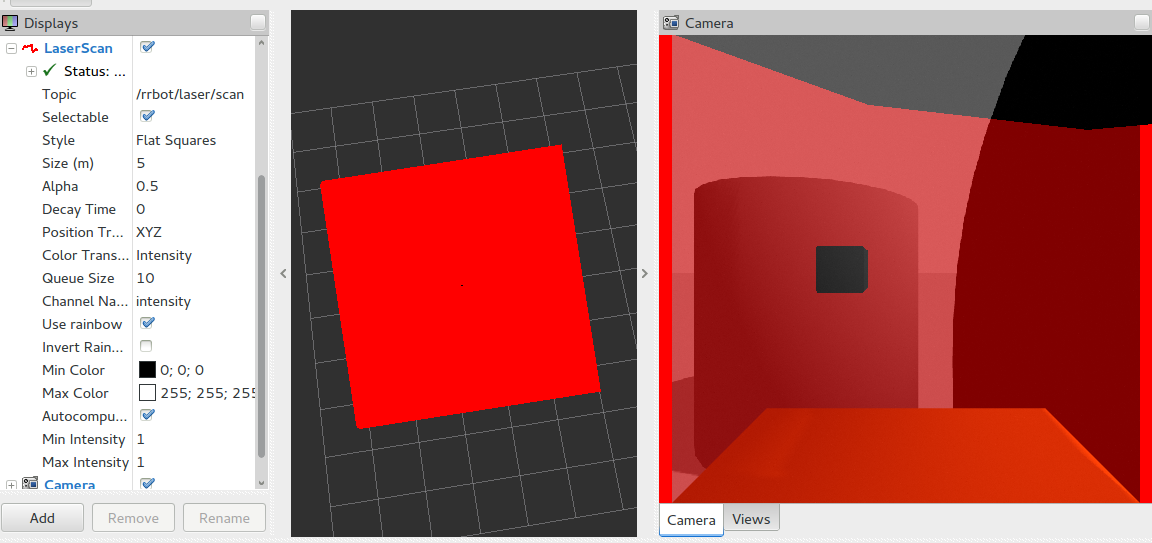
\includegraphics[width=0.75\textwidth]{img/screen_ue5_t2_laser.png}

\section{Task 3}\label{ass5_t3}

\begin{align*}
\alpha_1 &= 0 \\
d_1 &= L_1 \\
\Theta_1 &= 180 \pm \epsilon_{\Theta_1} \\
a_1 &= 0 \\
\\
\alpha_2 &= 90 \pm \epsilon_{\alpha_2} \\
d_2 &= 0 \\
\Theta_2 &= 45 \pm \epsilon_{\Theta_2} \\
a_2 &= 0 \\
\\
\alpha_3 &= 0 \\
d_3 &= 0 \\
\Theta_3 &= 45 \pm \epsilon_{\Theta_3} \\
a_3 &= L_2 \\
\\
\alpha_4 &= 90 \pm \epsilon_{\alpha_4} \\
d_4 &= d_4 \\
\Theta_4 &= 0 \pm \epsilon_{\Theta_4} \\
a_4 &= 0 \\
\\
\Theta_1 &= 180 \pm \epsilon_{\Theta_1} \\
\Theta_2 &= 45 \pm \epsilon_{\Theta_2} \\
\Theta_3 &= 45 \pm \epsilon_{\Theta_3} \\
\end{align*}
Annahme: Der Ursprung von Koordinatensystem 4 ist um $d_4$ vom Ursprung des Koordinatensystems 3 in der Tiefe ($d$) verschoben.
\begin{align*}
T_3^2(\alpha_2,a_2,\Theta_3,d_3) &= \left( \begin{matrix} cos(\Theta_{i}) & -sin(\Theta_i) & 0 & a_{i-1} \\ sin(\Theta_i) \cdot cos(\alpha_{i-1}) & cos(\Theta_i) \cdot cos(\alpha_{i-1}) & -sin(\alpha_{i-1}) & -sin(\alpha_{-1}) \cdot d_i \\ sin(\Theta_i) \cdot cos(\alpha_{i-1}) & cos(\Theta_i) \cdot sin(\alpha_{i-1}) & cos(\alpha_{i-1}) & cos(\alpha_{i-1}) \cdot d_i \\  0 & 0 & 0 & 1\end{matrix} \right) \\
T_3^2(\alpha_2,a_2,45,d_3) &= \left( \begin{matrix} cos(45) & -sin(45) & 0 & 0 \\ sin(45) \cdot cos(45) & cos(45) \cdot cos(45) & -sin(45) & -sin(90) \cdot 0 \\ sin(45) \cdot cos(90) & cos(45) \cdot sin(90) & cos(90) & cos(90) \cdot 0 \\  0 & 0 & 0 & 1\end{matrix} \right) \\
T_3^2(\alpha_2,a_2,45,d_3) &= \left( \begin{matrix} \frac{1}{\sqrt{2}} & -\frac{1}{\sqrt{2}} & 0 & 0 \\ \frac{1}{2} & \frac{1}{2} & -\frac{1}{\sqrt{2}} & 0 \\ 0 & \frac{1}{\sqrt{2}} & 0 & 0 \\  0 & 0 & 0 & 1\end{matrix} \right)
\end{align*}

\section{Task 4}\label{ass5_t4}

\subsection{a)}\label{ass5_t4a}

\begin{align*}
^{0}_3 A(q_1, q_2, q_3) &= ^{0}_1 A(q_1) \cdot ^{1}_2 A(q_2) \cdot ^{2}_3 A(q_3) \\
^{0}_3 A &= \left( \begin{matrix} cos(\Theta_1) & -sin(\Theta_1) & 0 & 0 \\ sin(\Theta_1) & cos(\Theta_1) & 0 & 0 \\ 0 & 0 & 1 & 0 \\ 0 & 0 & 0 & 1\end{matrix} \right) \cdot \left( \begin{matrix} 1 & 0 & 0 & 0 \\ 0 & 1 & 0 & 0 \\ 0 & 0 & 1 & d_2 \\ 0 & 0 & 0 & 1\end{matrix} \right) \cdot \left( \begin{matrix} 1 & 0 & 0 & 0 \\ 0 & 1 & 0 & 0 \\ 0 & 0 & 1 & d_3 \\ 0 & 0 & 0 & 1\end{matrix} \right) \\
^{0}_3 A &= \left( \begin{matrix} cos(\Theta_1) & -sin(\Theta_1) & 0 & 0 \\ sin(\Theta_1) & cos(\Theta_1) & 0 & 0 \\ 0 & 0 & 1 & d_2 \\ 0 & 0 & 0 & 1\end{matrix} \right) \cdot \left( \begin{matrix} 1 & 0 & 0 & 0 \\ 0 & 1 & 0 & 0 \\ 0 & 0 & 1 & d_3 \\ 0 & 0 & 0 & 1\end{matrix} \right) \\
^{0}_3 A &= \left( \begin{matrix} cos(\Theta_1) & -sin(\Theta_1) & 0 & 0 \\ sin(\Theta_1) & cos(\Theta_1) & 0 & 0 \\ 0 & 0 & 1 & d_2 + d_3 \\ 0 & 0 & 0 & 1\end{matrix} \right)
\end{align*}
Beschreibung der Koordinaten des Zielsystems:
\begin{align*}
f &: \mathbb{R}^3 \longrightarrow \mathbb{R}^3 \\
f &= B \\
B &= \left( \begin{matrix} cos(\Theta_1) & -sin(\Theta_1) & 0 \\ sin(\Theta_1) & cos(\Theta_1) & 0 \\ 0 & 0 & d_2 + d_3 \end{matrix} \right) \\
x &= cos(\Theta_1) - sin(\Theta_1) \\
y &= sin(\Theta_1) + cos(\Theta_1) \\
z &= d_2 + d_3
\end{align*}

\subsection{b)}\label{ass5_t4b}

\begin{align*}
\frac{x}{d \Theta_1} &= -sin(\Theta_1) - cos(\Theta_1)\\
\frac{x}{d d_2} &= 0 \\
\frac{x}{d d_3} &= 0 \\
\\
\frac{y}{d \Theta_1} &= -sin(\Theta_1) + cos(\Theta_1) \\
\frac{y}{d d_2} &= 0 \\
\frac{y}{d d_3} &= 0 \\
\\
\frac{z}{d \Theta_1} &= 0 \\
\frac{z}{d d_2} &= 1 \\
\frac{z}{d d_3} &= 1 \\
\end{align*}

\subsection{c)}\label{ass5_t4a}

\begin{align*}
J(q) &= \left( \begin{matrix} -sin(q_1)-cos(q_1) & -sin(q_1)+cos(q_1) & 0 \\ 0 & 0 & 1 \\ 0 & 0 & 1 \end{matrix} \right)
\end{align*}

  %\chapter{Assignment 6}\label{ass6}

\section{Task 1}\label{ass6_t1}

Siehe angehangene Dateien.

\section{Task 2}\label{ass6_t2}

Aufstellen und Ausrechnen der Gleichung:
\begin{align*}
\left( \begin{matrix} \frac{1}{2} \\ 0 \\ 1 \end{matrix} \right) &= \left( \begin{matrix} cos(\Theta_1) & sin(\Theta_1) & l_1 \\ -sin(\Theta_1) & cos(\Theta_1) & 0 \\ 0 & 0 & 1 \end{matrix} \right) \cdot \left( \begin{matrix} cos(\Theta_2) & sin(\Theta_2) & 0 \\ -sin(\Theta_2) & cos(\Theta_2) & 0 \\ 0 & 0 & 1 \end{matrix} \right) \cdot \left( \begin{matrix} l_2 \\ 0 \\ 1 \end{matrix} \right)
\end{align*}
Beschreibung der Lösungsmenge mit einer der beiden Ergebnisgleichungen:
\begin{align*}
nullspace \left( \left( \begin{matrix} \frac{1}{2} \\ x_2 \end{matrix} \right) \right) &= \left\lbrace \left( \begin{matrix}\Theta_1 \\ \Theta_2 \end{matrix} \right) | 2 \cdot cos(\Theta_1) + \frac{18}{10} \cdot cos(\Theta_1 + \Theta_2) -1 = 0 \right\rbrace\\
\end{align*}
Der Winkel $\Theta_1$ wird aus der Lösungsmenge gew\"ahlt.\\
Der Winkel $\Theta_2$ ist funktional abh\"angig vom Winkel $\Theta_1$:
\begin{align*}
\Theta_2 &= f(\Theta_1) \\
f(\Theta_1) &= -\Theta_1 \pm cos^{-1}(\Theta_1) \left( -\frac{20}{18} \cdot cos(\Theta_1) -\frac{10}{18} \right)
\end{align*}
Daraus ergibt sich:
\begin{align*}
nullspace \left( \left( \begin{matrix} \frac{1}{2} \\ x_2 \end{matrix} \right) \right) &= \left\lbrace \left( \begin{matrix}\Theta_1 \\ f(\Theta_1) \end{matrix} \right) | 2 \cdot cos(\Theta_1) + \frac{18}{10} \cdot cos(\Theta_1 + f(\Theta_1)) -1 = 0 \right\rbrace\\
\end{align*}
  %\chapter{Assignment 7}\label{ass7}

\section{Task 1}\label{ass7_t1}

\subsection{a}\label{ass7_t1a}

In the plots we used three colours to distinguish the results.\\
The blue lines are the current position on the y-axis, the red ones mark the deviation of the yaw and the cyan ones are the control output.\\

Plot for the P-controller with P set to 0.15:\\
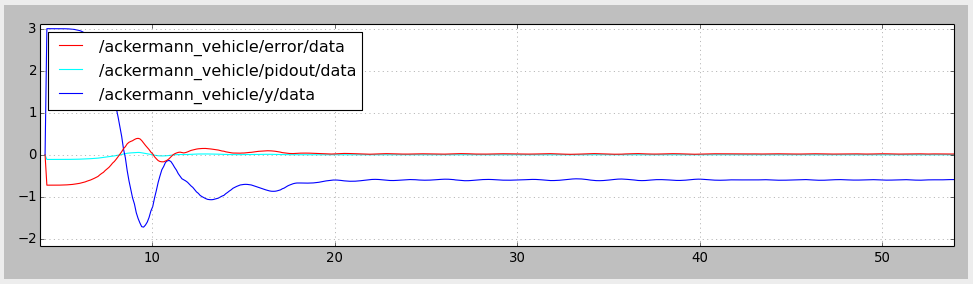
\includegraphics[width=0.75\textwidth]{img/screen_ue7_t1_p-015.png}

Plot for the PD-controller with 0.15(P) and 0.25(D):\\
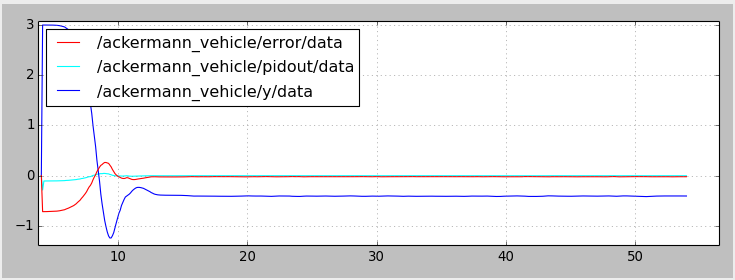
\includegraphics[width=0.75\textwidth]{img/screen_ue7_t1_p-015_d-025.png}

\subsection{b}\label{ass7_t1b}

Plot of P set to 0.05:\\
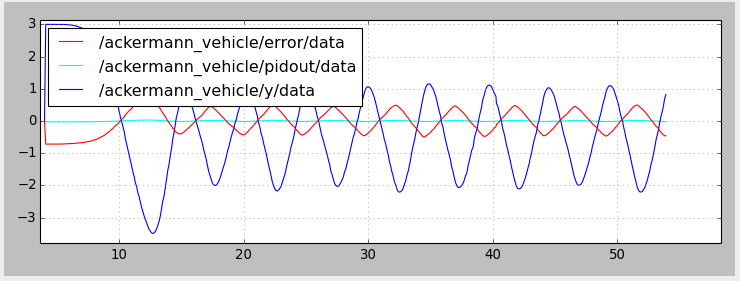
\includegraphics[width=0.75\textwidth]{img/screen_ue7_t2_p-005_osz.png}

As the system starts to oscillate at 0.05 and has a cycle of almost 5, the following equations determine the parameter for the PID-controller:\\
\begin{align*}
K_p &=0.6\cdot K_{p_k}      & = & 0.03\\
K_i &=\frac{2\cdot K_p}{t}  & = & 0.012\\
K_d &=0.12\cdot K_p\cdot t  & = & 0.018
\end{align*}\\

Plot of PID set to 0.03(P), 0.012(I) and 0.018(D):\\
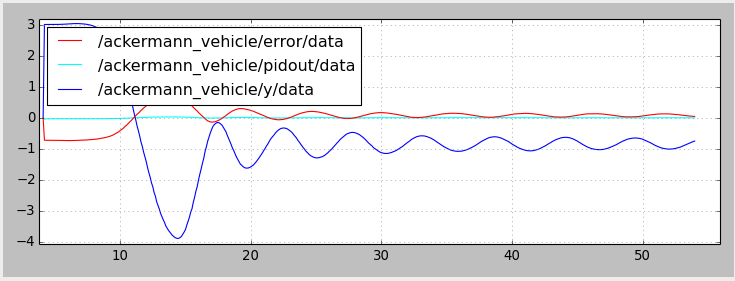
\includegraphics[width=0.75\textwidth]{img/screen_ue7_t2_pid.png}
  %\chapter{Assignment 8}\label{ass8}

\section{Task 1}\label{ass8_t1}

The following graphs will each represent one iteration of the hard A* variation on the given graph.\\
The green circles are nodes in the open list, red ones are in the closed list and the blue ones are unknown.

\noindent And the green numbers aside from the nodes are the original heuristic estimates, while the red numbers are the updated costs to reach that node and the red letter is the predecessor.

\definecolor {processblue}{cmyk}{0.96,0,0,0}
\definecolor {processred}{cmyk}{0,0.96,0,0}
\definecolor {processgreen}{cmyk}{0.96,0,0.96,0}
\tikzset{every label/.style={green}}
\tikzset{closed/.style={ circle ,top color =white , bottom color = processred!60 ,
draw,processred , text=blue , minimum width =1 cm}}
\tikzset{open/.style={ circle ,top color =white , bottom color = processgreen!60 ,
draw,processgreen , text=blue , minimum width =1 cm}}
\tikzset{state/.style ={ circle ,top color =white , bottom color = processblue!60 ,
draw,processblue , text=blue , minimum width =1 cm}}
\begin {center}
  \begin {tikzpicture}[- ,auto ,node distance = 2 cm and 3cm ,on grid ,
  semithick]
    \node[open,label={below:\small 19 \textcolor{red}{0}}] (H){h};
    \node[state,label={below:\small 1}] (G) [left = of H] {g};
    \node[state,label={below:\small 20}] (E) [right = of H] {e};
    \node[state,label={\small 42}] (C) [above right = of H] {c};
    \node[state,label={right:\small 35}] (D) [above left = of H] {d};
    \node[state,label={\small 0}] (A) [above left = of C] {a};
    \node[state,label={\small 9}] (B) [left = of D] {b};
    \node[state,label={below:\small 18}] (F) [left = of G] {f};
    \path (H) edge [left] node[below =0.15 cm] {10} (G);
    \path (H) edge [right] node[below =0.15 cm] {10} (E);
    \path (H) edge [left] node[above] {10} (C);
    \path (H) edge [left] node[below =0.15 cm] {10} (D);
    \path (E) edge [left] node[left =0.15 cm] {10} (C);
    \path (C) edge [left] node[below =0.15 cm] {10} (A);
    \path (G) edge [left] node[left =0.15 cm] {10} (D);
    \path (D) edge [left] node[below =0.15 cm] {10} (A);
    \path (D) edge [left] node[below =0.15 cm] {10} (B);
    \path (G) edge [left] node[below =0.15 cm] {10} (F);
    \path (F) edge [right] node[left =0.15 cm] {10} (B);
    \path (B) edge [left] node[above =0.15 cm] {10} (A);
  \end{tikzpicture}
\end{center}

\begin {center}
  \begin {tikzpicture}[- ,auto ,node distance = 2 cm and 3cm ,on grid ,
  semithick]
    \node[closed,label={below:\small 19 \textcolor{red}{0}}] (H){h};
    \node[open,label={below:\small 1 \textcolor{red}{11 h}}] (G) [left = of H] {g};
    \node[open,label={below:\small 20 \textcolor{red}{30 h}}] (E) [right = of H] {e};
    \node[open,label={\small 42 \textcolor{red}{52 h}}] (C) [above right = of H] {c};
    \node[open,label={right:\small 35 \textcolor{red}{45 h}}] (D) [above left = of H] {d};
    \node[state,label={\small 0}] (A) [above left = of C] {a};
    \node[state,label={\small 9}] (B) [left = of D] {b};
    \node[state,label={below:\small 18}] (F) [left = of G] {f};
    \path (H) edge [left] node[below =0.15 cm] {10} (G);
    \path (H) edge [right] node[below =0.15 cm] {10} (E);
    \path (H) edge [left] node[above] {10} (C);
    \path (H) edge [left] node[below =0.15 cm] {10} (D);
    \path (E) edge [left] node[left =0.15 cm] {10} (C);
    \path (C) edge [left] node[below =0.15 cm] {10} (A);
    \path (G) edge [left] node[left =0.15 cm] {10} (D);
    \path (D) edge [left] node[below =0.15 cm] {10} (A);
    \path (D) edge [left] node[below =0.15 cm] {10} (B);
    \path (G) edge [left] node[below =0.15 cm] {10} (F);
    \path (F) edge [right] node[left =0.15 cm] {10} (B);
    \path (B) edge [left] node[above =0.15 cm] {10} (A);
  \end{tikzpicture}
\end{center}

\begin {center}
  \begin {tikzpicture}[- ,auto ,node distance = 2 cm and 3cm ,on grid ,
  semithick]
    \node[closed,label={below:\small 19 \textcolor{red}{0}}] (H){h};
    \node[closed,label={below:\small 1 \textcolor{red}{11 h}}] (G) [left = of H] {g};
    \node[open,label={below:\small 20 \textcolor{red}{30 h}}] (E) [right = of H] {e};
    \node[open,label={\small 42 \textcolor{red}{52 h}}] (C) [above right = of H] {c};
    \node[open,label={right:\small 35 \textcolor{red}{45 h}}] (D) [above left = of H] {d};
    \node[state,label={\small 0}] (A) [above left = of C] {a};
    \node[state,label={\small 9}] (B) [left = of D] {b};
    \node[open,label={below:\small 18 \textcolor{red}{38 g}}] (F) [left = of G] {f};
    \path (H) edge [left] node[below =0.15 cm] {10} (G);
    \path (H) edge [right] node[below =0.15 cm] {10} (E);
    \path (H) edge [left] node[above] {10} (C);
    \path (H) edge [left] node[below =0.15 cm] {10} (D);
    \path (E) edge [left] node[left =0.15 cm] {10} (C);
    \path (C) edge [left] node[below =0.15 cm] {10} (A);
    \path (G) edge [left] node[left =0.15 cm] {10} (D);
    \path (D) edge [left] node[below =0.15 cm] {10} (A);
    \path (D) edge [left] node[below =0.15 cm] {10} (B);
    \path (G) edge [left] node[below =0.15 cm] {10} (F);
    \path (F) edge [right] node[left =0.15 cm] {10} (B);
    \path (B) edge [left] node[above =0.15 cm] {10} (A);
  \end{tikzpicture}
\end{center}

\begin {center}
  \begin {tikzpicture}[- ,auto ,node distance = 2 cm and 3cm ,on grid ,
  semithick]
    \node[closed,label={below:\small 19 \textcolor{red}{0}}] (H){h};
    \node[closed,label={below:\small 1 \textcolor{red}{11 h}}] (G) [left = of H] {g};
    \node[closed,label={below:\small 20 \textcolor{red}{30 h}}] (E) [right = of H] {e};
    \node[open,label={\small 42 \textcolor{red}{52 h}}] (C) [above right = of H] {c};
    \node[open,label={right:\small 35 \textcolor{red}{45 h}}] (D) [above left = of H] {d};
    \node[state,label={\small 0}] (A) [above left = of C] {a};
    \node[state,label={\small 9}] (B) [left = of D] {b};
    \node[open,label={below:\small 18 \textcolor{red}{38 g}}] (F) [left = of G] {f};
    \path (H) edge [left] node[below =0.15 cm] {10} (G);
    \path (H) edge [right] node[below =0.15 cm] {10} (E);
    \path (H) edge [left] node[above] {10} (C);
    \path (H) edge [left] node[below =0.15 cm] {10} (D);
    \path (E) edge [left] node[left =0.15 cm] {10} (C);
    \path (C) edge [left] node[below =0.15 cm] {10} (A);
    \path (G) edge [left] node[left =0.15 cm] {10} (D);
    \path (D) edge [left] node[below =0.15 cm] {10} (A);
    \path (D) edge [left] node[below =0.15 cm] {10} (B);
    \path (G) edge [left] node[below =0.15 cm] {10} (F);
    \path (F) edge [right] node[left =0.15 cm] {10} (B);
    \path (B) edge [left] node[above =0.15 cm] {10} (A);
  \end{tikzpicture}
\end{center}

\begin {center}
  \begin {tikzpicture}[- ,auto ,node distance = 2 cm and 3cm ,on grid ,
  semithick]
    \node[closed,label={below:\small 19 \textcolor{red}{0}}] (H){h};
    \node[closed,label={below:\small 1 \textcolor{red}{11 h}}] (G) [left = of H] {g};
    \node[closed,label={below:\small 20 \textcolor{red}{30 h}}] (E) [right = of H] {e};
    \node[open,label={\small 42 \textcolor{red}{52 h}}] (C) [above right = of H] {c};
    \node[open,label={right:\small 35 \textcolor{red}{45 h}}] (D) [above left = of H] {d};
    \node[state,label={\small 0}] (A) [above left = of C] {a};
    \node[open,label={\small 9 \textcolor{red}{39 f}}] (B) [left = of D] {b};
    \node[closed,label={below:\small 18 \textcolor{red}{38 g}}] (F) [left = of G] {f};
    \path (H) edge [left] node[below =0.15 cm] {10} (G);
    \path (H) edge [right] node[below =0.15 cm] {10} (E);
    \path (H) edge [left] node[above] {10} (C);
    \path (H) edge [left] node[below =0.15 cm] {10} (D);
    \path (E) edge [left] node[left =0.15 cm] {10} (C);
    \path (C) edge [left] node[below =0.15 cm] {10} (A);
    \path (G) edge [left] node[left =0.15 cm] {10} (D);
    \path (D) edge [left] node[below =0.15 cm] {10} (A);
    \path (D) edge [left] node[below =0.15 cm] {10} (B);
    \path (G) edge [left] node[below =0.15 cm] {10} (F);
    \path (F) edge [right] node[left =0.15 cm] {10} (B);
    \path (B) edge [left] node[above =0.15 cm] {10} (A);
  \end{tikzpicture}
\end{center}

\begin {center}
  \begin {tikzpicture}[- ,auto ,node distance = 2 cm and 3cm ,on grid ,
  semithick]
    \node[closed,label={below:\small 19 \textcolor{red}{0}}] (H){h};
    \node[closed,label={below:\small 1 \textcolor{red}{11 h}}] (G) [left = of H] {g};
    \node[closed,label={below:\small 20 \textcolor{red}{30 h}}] (E) [right = of H] {e};
    \node[open,label={\small 42 \textcolor{red}{52 h}}] (C) [above right = of H] {c};
    \node[open,label={right:\small 35 \textcolor{red}{45 h}}] (D) [above left = of H] {d};
    \node[open,label={\small 0 \textcolor{red}{40 b}}] (A) [above left = of C] {a};
    \node[closed,label={\small 9 \textcolor{red}{39 f}}] (B) [left = of D] {b};
    \node[closed,label={below:\small 18 \textcolor{red}{38 g}}] (F) [left = of G] {f};
    \path (H) edge [left] node[below =0.15 cm] {10} (G);
    \path (H) edge [right] node[below =0.15 cm] {10} (E);
    \path (H) edge [left] node[above] {10} (C);
    \path (H) edge [left] node[below =0.15 cm] {10} (D);
    \path (E) edge [left] node[left =0.15 cm] {10} (C);
    \path (C) edge [left] node[below =0.15 cm] {10} (A);
    \path (G) edge [left] node[left =0.15 cm] {10} (D);
    \path (D) edge [left] node[below =0.15 cm] {10} (A);
    \path (D) edge [left] node[below =0.15 cm] {10} (B);
    \path (G) edge [left] node[below =0.15 cm] {10} (F);
    \path (F) edge [right] node[left =0.15 cm] {10} (B);
    \path (B) edge [left] node[above =0.15 cm] {10} (A);
  \end{tikzpicture}
\end{center}

\noindent Now the first node in the open list is a, so we stop A* and can extract the resulting path vie the predecessors starting with the node a.\\
The resulting path would be: h $\rightarrow$ g $\rightarrow$ f $\rightarrow$ b $\rightarrow$ a with the total costs of 40, which obviously are twice as much as those of the optimal path.

\subsection{Task 2}\label{ass8_t2}

In the following plots, as in the assignment sheet, the green dots are the obstacles, the red one is the target, the blue one is the start, grey ones are nodes in the open-list, purple ones are in the closed-list and the yellow line is the path calculated.\\

Plot for i=-1:\\
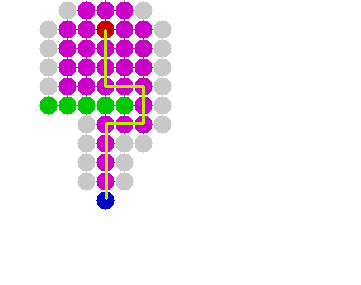
\includegraphics[width=0.5\textwidth]{img/screen_ue8_t2-1.png}\newpage
Plot for i=0:\\
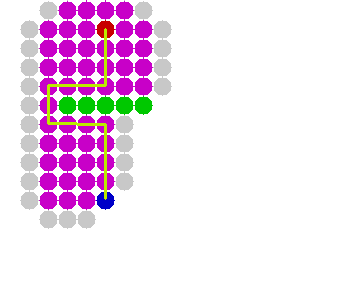
\includegraphics[width=0.5\textwidth]{img/screen_ue8_t2-2.png}\\
Plot for i=1:\\
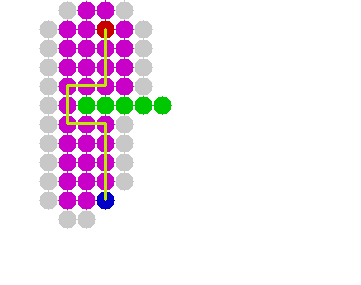
\includegraphics[width=0.5\textwidth]{img/screen_ue8_t2-3.png}
  %\chapter{Assignment 12}\label{ass12}

\section{Task 1}\label{ass12_t1}

\subsection{a)}

Gesucht sind die Parameter $a,b,c,d,h,i,j,k$ für zwei Splines $f\mathopen[0,1 \mathclose]\rightarrow \mathbb{R} ,g\mathopen[1,2\mathclose]\rightarrow \mathbb{R}$. Die gesuchten Funktionen mit ihren Ableitungen sind

\begin{align}
f(x) &=a \cdot x^3+b \cdot x^2+c \cdot x+d \\
f'(x) &= 3 \cdot a \cdot x^2+2 \cdot b \cdot x+c \\
f''(x) &= 6 \cdot a \cdot x+2 \cdot b \\
g(x)&=h\cdot x^3+i\cdot x^2+j\cdot x+k \\
g'(x)&=3\cdot h\cdot x^2+2\cdot i\cdot x+j \\	
g''(x)&=6\cdot h\cdot x+2\cdot i \\
\end{align}
Aus der Beschreibung sind direkt die folgenden Eigenschaften abzulesen
\begin{align}
f(0) &= 0 \\
f'(0) &= 0 \\
g(2) &= 8 \\
g'(2) &= 8 \\
f''(1) &= 0 \\
g''(1) &= 0 \\
\end{align}
Um das soweit unterbestimmte Gleichungssystem lösen zu können, verwenden wir als zusätzliche Eigenschaft die Tatsache, dass sich $f$ und $g$ an der Grenze ihrer Definitionsbereiche bei $x=1$ schneiden müssen. Es gilt also zusätzlich
\begin{align}
f(1) &= g(1)\\
f'(1) &= g'(1)
\end{align}
Ausformuliert erhält man somit ein lineares Gleichungssystem
\begin{align}
d &= 0\\
k &= 0\\
8 \cdot h+4 \cdot i+2 \cdot j &= 8 \\
12 \cdot h+4 \cdot i+j &= 8 \\
6 \cdot a+2 \cdot b &= 0 \\
6 \cdot h+2 \cdot i &= 0 \\
a+b+c &= h+i+j \\
3 \cdot a+2 \cdot b+c &= 3 \cdot h+2 \cdot i+j \\
\end{align}
$d,k$ sind also an dieser Stelle bereits bekannt. Für die übrigen Parameter lösen wir mittels Gaussschem Eliminierungsverfahren:
\begin{center}
\begin{tabular}{ccccccc}
$a$&$b$&$c$&$h$&$i$&$j$&$=$\\
\hline
0&0&0&8&4&2&8 \\
0&0&0&12&4&1&8 \\
6&2&0&0&0&0&0 \\
0&0&0&6&2&0&0 \\
1&1&1&-1&-1&-1&0 \\
3&2&1&-3&-2&-1&0
\end{tabular}
\end{center}
Zuerst etwas umsortieren
\begin{center}
\begin{tabular}{ccccccc}
$a$&$b$&$c$&$h$&$i$&$j$&$=$ \\
\hline
1&1&1&-1&-1&-1&0 \\
3&2&1&-3&-2&-1&0 \\
6&2&0&0&0&0&0 \\
0&0&0&6&2&0&0 \\
0&0&0&8&4&2&8 \\
0&0&0&12&4&1&8
\end{tabular}
\end{center}
$a$-Spalte eliminieren
\begin{center}
\begin{tabular}{ccccccc}
$a$&$b$&$c$&$h$&$i$&$j$&$=$\\
\hline
1&1&1&-1&-1&-1&0 \\
0&-1&-2&0&1&2&0 \\
0&-4&-6&6&6&6&0 \\
0&0&0&6&2&0&0 \\
0&0&0&8&4&2&8 \\
0&0&0&12&4&1&8
\end{tabular}
\end{center}
$b$-Spalte eliminieren
\begin{center}
\begin{tabular}{ccccccc}
$a$&$b$&$c$&$h$&$i$&$j$&$=$\\
\hline
1&1&1&-1&-1&-1&0 \\
0&1&2&0&-1&-2&0 \\
0&0&2&6&2&-2&0 \\
0&0&0&6&2&0&0 \\
0&0&0&8&4&2&8 \\
0&0&0&12&4&1&8
\end{tabular}
\end{center}
$c$-Spalte sieht schon gut aus, deshalb weiter mit $h$
\begin{center}
\begin{tabular}{ccccccc}
$a$&$b$&$c$&$h$&$i$&$j$&$=$ \\
\hline
1&1&1&-1&-1&-1&0 \\
0&1&2&0&-1&-2&0 \\
0&0&1&3&1&-1&0 \\
0&0&0&6&2&0&0 \\
0&0&0&0&4&6&24 \\
0&0&0&0&0&1&8 \\
\end{tabular}
\end{center}
So ein Glück $i,j$ ergeben sich direkt! Von unten nach oben können nun alle Parameter ausgerechnet werden, zu
\begin{align}
&a=2,b=-6,c=8,\\
&h=2,i=-6,j=8
\end{align}
Eine partielle Interpolation war hier also gar nicht nötig - ein einziges Polynom $e\mathopen[0,2\mathclose]\rightarrow \mathbb{R}$ genügt, um alle Eigenschaften zu erfüllen.\\
\\
Ergebnis:
$$e(x)=2 \cdot x^3-6 \cdot x^2+2 \cdot x$$

\subsection{b)}
Auch wenn $f=g=e$ sind hier unabhängig von einander $f$ in blau und $g$ in rot geplottet (Abbildung \ref{fig1}).

\begin{figure}[!htpb]
\centering
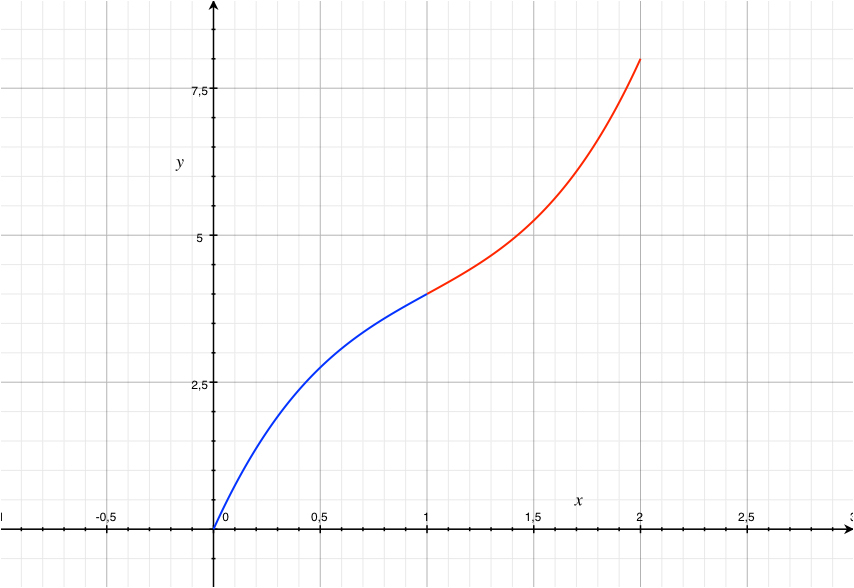
\includegraphics[width=\linewidth]{img/capture_1-1.jpg}
\caption{Spline}
\label{fig1}
\end{figure}

\subsection{c)}

Der Schnittpunkt $(x_s,y_s)$ ist vorgegeben bei $x_s=1$ mit
$y_s=e(1)=a+b+c=4$
Die Geschwindigkeit $v$ ist dort
$v=e'(1)=3\cdot a+2\cdot b+c=2$


\subsection{Task 3}\label{ass12_t3}

\subsection{a)}

Wir definieren Ereignis $A$ als "keine Enten sind zu sehen" und Ereignis $B$ als "Krokodile sind zu sehen".\\
Wir wissen $P(\neg A) = (P(\neg A| B) + P(\neg A | \neg B)) = (0.1+0.5) = 0.6$.\\
Daraus folgt $P(A) = 1 - P(l\not A) = 0.4$\\
Außerdem wissen wir $P(B) = P(\neg A | B) + P(A | B)$.\\
Das stellen wir um nach $P(A|B) = P(B) - P(\neg A | B)$ und rechnen aus $P(A|B) = 0.2 - 0.03 = 0.17$.\\
\\
Weil wir alle benötigten Variablen haben, setzen wir in den Satz von Bayes ein
Es gilt der Satz von Bayes $P(B|A) = \frac{P(A|B) \cdot P(B)}{P(A)} = \frac{0.17 \cdot 0.2}{0.4} = 0.085$.

\subsection{b)}
Die Variablen $\neg A$ und $B$ sind abhängig.\\
\\
Beweis durch Widerspruch:\\
\\
Angenommen $\neg A$ und $B$ sind unabhängig, dann gilt $P(\neg A|B) = P(\neg A)$.
\\
$0.1 \neq 0.6$ Widerspruch $q.e.d.$



  \chapter{Assignment 13}\label{ass13}

\subsection{Task 3}\label{ass13_t3}

\begin{figure}[!htpb]
\centering
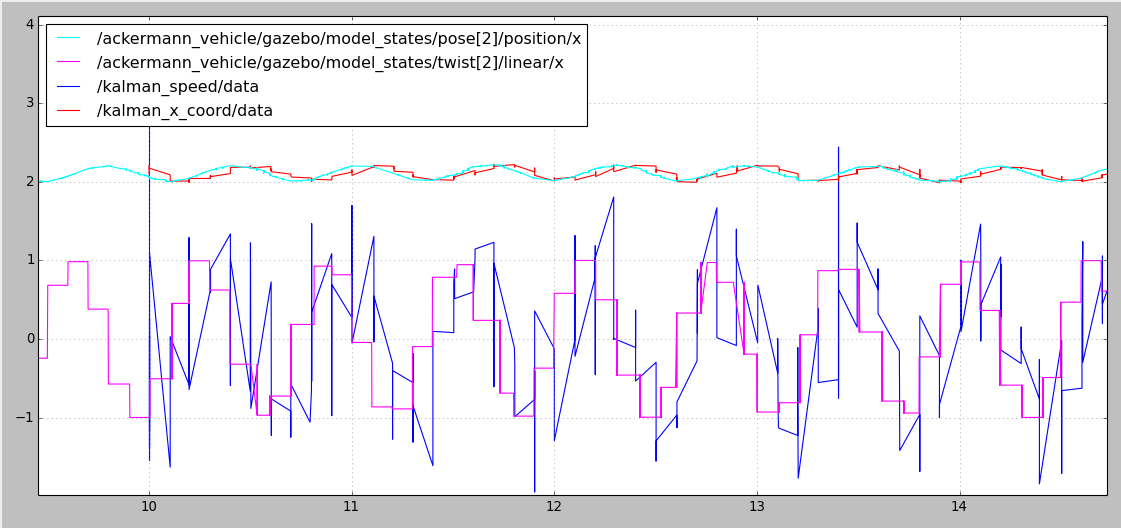
\includegraphics[width=\linewidth]{img/screen_ue13_t3.png}
\caption{Plot}
\label{fig1}
\end{figure}
\end{document}